% Basic security concepts
\chapter{Network Security Concepts}
First of all, lets try to define what is \textit{network security}. Well, of course it depends 
on the context, but in general:
\begin{boxH}
  \textbf{Network security} is defined as the \textit{protection} of networks and their services from unauthorized
  modification, destruction, or disclosure.
\end{boxH}
It provides assurance hat the network performs as expected and in a correct way, with no unexpected 
side effects.\\
Network security focuses mainly on networks, network protocols, and network applications, but it 
also includes all the networks devices and the physical infrastructure.
\begin{subsubsection}{Security Threats}
  While traditional networks have no limitations on the coverage, wireless ones have, and its binded
  to the broadcast radio channel.\\
  Wireless networks require decentralized medium access mechanism in medium access
  control (MAC) layer, while also including the means to deal with the mobility of the users.\\
  For those issues, wireless networks make it up with the flexibility and mobility they provide.\\
  Furthermore, the surface of attack is much larger, because the radio waves can be intercepted
  from anywhere in range.\\
  To sum it up, it has many advantages, but also many issues that need to be addressed.
\end{subsubsection}
\begin{section}{Security attacks}
  Security is all about dealing with threats and risk, but ideally the system should be designed 
  to address and prevent all possible attacks, but it is not always, or to be honest, almost never possible.\\
  If prevention is not possible, a solution is to detect the attack and then recover from it.\\
  Recall also that an attack is a deliberate action to exploit a vulnerability, which is a 
  \textit{weakness} of a system.\\
  Attacks are formally classified as \textbf{passive attacks} and \textbf{active attacks}:
  \begin{itemize}
    \item Passive attack: the attacker can only read data/traffic
      \subitem \textit{Example}: eavesdropping, can be countered with encryption
      \subitem \textit{Example}: traffic analysis
    \item Active attacker: the attacker can also modify, delete, or create data/traffic
      \subitem \textit{Example}: masquerade, an attacker pretends to be some other entity, usually 
      an authorized user. Can be countered with authentication.
      \subitem \textit{Example}: replay, an attacker first captures a message, (encrypted or not),
      then replays this message to its designated receiver, can be countered with serialization.
      \subitem \textit{Example}: modification of messages, can be countered with integrity of the 
      data, peer authentication, encryption, and serialization(?).
      \subitem \textit{Example}: denial of service
  \end{itemize}
  \begin{figure}[h]
    \centering
    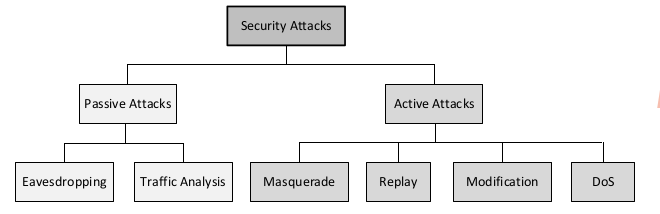
\includegraphics[width=0.7\textwidth]{img/wireless/attacks classification.png}
    \caption{General classification if attacks}
  \end{figure}

  Passive attacks are much harder to detect, because there is no data alteration or system
  manipulation.

\end{section}
\begin{section}{Security Services and proprieties}
  \begin{boxH}
    \textbf{Security services} are the features in a system designed against possible attacks.
  \end{boxH}
  The National Institute of Standards and Technology (NIST) computer security handbook introduces 
  three key security services: confidentiality, integrity, and availability.\\
  We will go over them and some more in the following paragraphs.
  \begin{paragraph}{Access Control}
    Access control is the process of determining what permissions a user should have, and what 
    resources they can access.\\
    this is because the serve should only be accessed by authorized users, and the data should only
    be accessed by authorized users.
  \end{paragraph}
  \begin{paragraph}{Authentication}
    Authentication is the process of verifying the identity of a user.\\
    The goal is to ensure that the user is who they claim to be.
  \end{paragraph}
  \begin{paragraph}{Confidentiality}
    Confidentiality is the process of ensuring that data is only accessible to those who are authorized
    to access it.\\
    This is usually done by encrypting the data.
  \end{paragraph}
  \begin{paragraph}{Integrity}
    Integrity is the process of ensuring that data is not altered in transit.\\
    This is usually done by using checksums or digital signatures.
  \end{paragraph}
  \begin{paragraph}{Non-repudiation}
    Non-repudiation is the process of ensuring that a user cannot deny that they performed a 
    particular action.\\
    This is usually done by using digital signatures.
  \end{paragraph}
  \begin{paragraph}{Availability}
    Availability is the process of ensuring that a system is available when it is needed.\\
    This is usually done by using redundancy and failover systems.
  \end{paragraph}

\end{section}
\begin{section}{Security Mechanisms}
  \begin{boxH}
    Security mechanisms are methods to achieve security services in a system.\\
    They can be implemented in hardware, software, or a combination of both.
  \end{boxH}
  x.800 defines a set of security mechanisms that can be used to achieve the security services
  we talked about before:
  \begin{itemize}
    \item Encryption
    \item Authentication
    \item Access Control
    \item Digital Signatures
    \item Data integrity
    \item Traffic Padding and Routing Control
    \item Notarization
  \end{itemize}
  \begin{paragraph}{Encryption}
    Encryption is the process of encoding data so that only authorized users can read it.\\
    It can provide confidentiality for either data or traffic flow information and can play a part 
    in or complement several other security mechanisms
  \end{paragraph}
  \begin{paragraph}{Authentication}
    In this context, authentication is applied to the message or a party of the communication.\\
  \end{paragraph}
  \begin{paragraph}{Access Control}
    It is applied to determine and enforce the access rights of the entity depending on the 
    authenticated identity of an entity or information about the entity (such as membership in a 
    known set of entities) or capabilities of the entity.
  \end{paragraph}
  \begin{paragraph}{Digital Signatures}
    This mechanism is used to provide integrity and non-repudiation.
  \end{paragraph}
  \begin{paragraph}{Traffic Padding and Routing Control}
    It can be used to provide various levels of protection against traffic analysis.
  \end{paragraph}
  \begin{paragraph}{Notarization}
    It can be used to provide non-repudiation, and also certificate the destination.
  \end{paragraph}
\end{section}
\begin{section}{Levels of impact}
  The impact of a security breach can be classified into three levels:
  \begin{itemize}
    \item Low impact: the breach has little or no effect on the assets, operations or individuals.
    \item Moderate impact: the breach has a noticeable effect on the system or the data.
    \item High impact: the breach has severe or catastrophic effects on the system or the data.
  \end{itemize}
\end{section}

